\chapter{Design and Implementation of Our Approach}
\label{chap:ourapproach}
\todo{This chapter lays out the design and architecture of our Windows kernel driver.}\\
\todo{Where there were multiple ways to do things, we will provide the reasons behind our choice.}\\
\todo{This includes the choice for WDM as the used framework for the driver.}

\section{Rejected Driver Frameworks}
\label{chap:ourapproach.rejected}
As already mentioned in \autoref{chap:background.kerneldriver.wdm}, there are different frameworks to choose from when writing a driver. In this section, we will discuss some other frameworks that we ultimately did not use for our driver, even though we implemented an early prototype using one of them.

\subsection{The Filter Manager}
\label{chap:ourapproach.rejected.fltmgr}
The filter manager is a kernel driver that ships with Windows, implementing commonly required functionality to simplify the development of third-party file system filter drivers. Filter drivers that make use of the filter manager are called \emph{minifilter drivers}. They can, among other things, filter IRPs by registering a pre- and/or postoperation callback routine. These are the equivalents to WDM's dispatch and completion routines. Just like the I/O manager for WDM drivers, the filter manager is responsible for calling a minifilter's appropriate callback routine when an IRP arrives \cite{Fltmgr}.

Also similar to WDM drivers, the order in which an IRP passes through multiple minifilters is deterministic and configurable. It depends on the minifilters' \emph{altitude}, which is a value between 40,000 and 429,999.\footnote{\label{fn:ourapproach.rejected.altitudevalues} Lower altitudes are also possible, but are reserved by Windows for internal use.} For preoperation callbacks, a driver with a higher altitude is called before a driver with a lower altitude, and vice versa for postoperation callbacks. There are pre-defined groups of altitude values, called \emph{load order groups}. Examples are the Anti-Virus group (using an altitude between 320,000 and 329,999) and the Encryption group (140,000 to 149,999). To ensure that all minifilters have an appropriate altitude, Microsoft is responsible for assigning altitude values\footnote{\label{fn:ourapproach.rejected.assignedaltitudes} At \url{https://docs.microsoft.com/en-us/windows-hardware/drivers/ifs/allocated-altitudes} one can browse a list of all currently assigned altitudes.} \cite{Fltmgr}.

During the development process of our driver, we implemented a first prototype which used the filter manager. It worked to some extent, but ultimately it was not fit for its purpose. The architecture of an I/O stack that includes the filter manager shown in \autoref{fig:ourapproach.rejected.fltmgr} explains why this is the case: the filter manager and therefore all minifilters always sit above the file system driver. LUKS2 encryption however sits below the file system, meaning that despite our minifilter the file system driver can only read the encrypted data. We did not notice this during development because we used raw I/O to test our driver. This means that we created a handle to a path like \texttt{\textbackslash Device\textbackslash HarddiskVolume6} and performed I/O using that. Interestingly, in this case our minifilter successfully decrypted reads from the volume. %But the file system driver still could not recognize the file system. 

\begin{figure}
	\center
	\small
	\begin{tikzpicture}
		\node at (2, 8.7) (usr) {User request for file I/O};

		\node[anchor=east] at (9.45, 8.45) {\footnotesize User mode};
		\draw[dashed] (-0.5, 8.2) -- (9.5, 8.2);
		\node[anchor=east] at (9.45, 7.95) {\footnotesize Kernel mode};

		\node[rect, fill=tPink, from={0, 6.4 to 4, 7.7}] (io)  {I/O manager};
		\node[rect, fill=tOrng, from={0, 3.2 to 4, 4.5}] (flt) {Filter manager};
		\node[rect, fill=tGren, from={0, 0   to 4, 1.3}] (fs)  {File system driver};

		\node[rect, fill=tYlow, from={5.5, 4.7 to 8.5, 6}]   (mfa) {Minifilter A\\\footnotesize Altitude 365000};
		\node[rect, fill=tYlow, from={5.5, 3.2 to 8.5, 4.5}] (mfb) {Minifilter B\\\footnotesize Altitude 325000};
		\node[rect, fill=tYlow, from={5.5, 1.7 to 8.5, 3}]   (mfc) {Minifilter C\\\footnotesize Altitude 305000};

		\node[rect, fill=tLblu, from={5, 0 to 9, 1.3}] (sto) {Storage device stack};

		\draw[arrow] (usr.south) -> (io.north);
		\draw[arrow] (io.south)  -> (flt.north);
		\draw[<->] (flt.east) + (0, 0.325)  -- +(0.75, 0.325)  |- (mfa.west);
		\draw[<->] (flt.east)               -- +(0.75, 0)      |- (mfb.west);
		\draw[<->] (flt.east) + (0, -0.325) -- +(0.75, -0.325) |- (mfc.west);
		\draw[arrow] (flt.south) -> (fs.north);
		\draw[arrow] (fs.east)   -> (sto.west);
	\end{tikzpicture}
	\caption[
		Example of a filter manager I/O stack
	]{
		Example of a filter manager I/O stack (modified after \cite{Fltmgr}). A user initiates an I/O request, which the I/O manager receives first and forwards to the file system. The filter manager intercepts the request and lets it pass through the registered minifilters, in order according to their altitude (their altitude places them in the following groups, ordered from A to C: Activity Monitor, Anti-Virus, and Replication). After this, the file system driver processes the request and translates it from file-based to something that a driver in the storage device's stack can understand. Finally, this device stack receives the request from the file system driver.
	}
	\label{fig:ourapproach.rejected.fltmgr}
\end{figure}

We figured out why the decrypted file system was not recognized by Windows through debugging with WinDbg. Online research yielded the name of the driver responsible for recognizing FAT filesystems (our test LUKS2 volume contained a FAT32 filesystem): \texttt{fsrec.sys}. Using information from unofficial online documentation,\footnote{\label{fn:ourapproach.rejected.fsrecdoc} \url{http://www.codewarrior.cn/ntdoc/win2k/fsrec/index.htm}} we set a breakpoint at \texttt{fsrec}'s \texttt{IsFatVolume} routine. It receives the first sector of a volume and determines whether this matches the format of a FAT boot sector. When hitting the breakpoint and dumping the value of the function's parameter in WinDbg, it became clear that this routine received the encrypted first sector of the LUKS2 volume, consequently (and correctly) classifying it as a non-FAT volume.

See the official documentation \cite{Fltmgr} for more information on the filter manager and minifilter drivers.

\todo{\href{https://docs.microsoft.com/en-us/windows-hardware/drivers/ifs/how-file-system-filter-drivers-are-different-from-device-drivers}{this} and \href{https://docs.microsoft.com/en-us/windows-hardware/drivers/ifs/how-file-system-filter-drivers-are-similar-to-device-drivers}{this}?}

\subsection{The Windows Driver Frameworks}
\label{chap:ourapproach.rejected.wdf}
As already mentioned in \autoref{chap:background.kerneldriver.wdm}, another possibility to develop a driver are the Kernel Mode Driver Framework (KMDF) and User Mode Driver Framework (UMDF), together called the Windows Driver Frameworks (WDF). These try to simplify things by abstracting away some of the details that WDM drivers have to care about. The basic principles (e.g. IRP-based I/O) remain the same \cite{Yosifovich2017}.

We decided against using UMDF out of performance concerns; as the framework's name suggests, UMDF drivers run in user mode. This has certain advantages, such as increased system stability. But most of the I/O ecosystem runs in kernel mode, which means that switches between kernel and user mode are necessary when an I/O driver runs in user mode. These induce latency, together with some additional communication with the kernel \cite{Yosifovich2017}.

KMDF does not have this problems, but there were other factors that led to our decision against it:
\begin{itemize}
	\item We had previously tried another framework that simplified things though abstraction (see \autoref{chap:ourapproach.rejected.fltmgr}) and it had not worked. Therefore it seemed safer to do all the work ourselves, and in return be sure that the framework will not be a reason for failure.
	\item By default, KMDF filter drivers pass all received IRPs to the next driver in the stack \cite{Wdf}. However, our planned approach was as follows: don't pass through anything at first, and then gradually during the development process allow more and more requests to pass through. This is still possible with KMDF, but more work than for a WDM driver.
	\item One of the biggest selling points of using KMDF is that it handles PnP and Power IRPs for the driver. These are not really relevant to filter drivers, though (see \todo{\autoref{chap:ourapproach.final.otherrequests}} for how our final driver handles them). Therefore we would not gain that much by sacrificing total control for reduced complexity, because the hidden complexity is not that relevant in the first place.
	\item Finally, writing a WDM driver requires a more complete understanding of how the kernel's IRP-based I/O system works. We wanted to learn as much as possible, and for this purpose WDM seemed the better fit.
\end{itemize}

Now that our WDM driver is finished, it would be interesting to compare it to an equivalent that was written using KMDF, both its architecture and performance. This is left as an exercise to the curious reader; \autoref{chap:ourapproach.final} should be a good starting point.

\cite{Yosifovich2017} contains detailed information on the architecture and inner workings of both KMDF and UMDF. The official documentation \cite{Wdf} is also a valuable source of information.

\subsection{Other User Space Frameworks}
\label{chap:ourapproach.rejected.other}
There also exist third-party user mode libraries for developing file system drivers, e.g. \url{https://github.com/billziss-gh/winfsp} or \url{https://github.com/dokan-dev/dokany}. However, these probably suffer the same drawbacks as UMDF drivers, and were therefore rejected.

\section{The Final WDM Driver}
\label{chap:ourapproach.final}
After deciding against the frameworks mentioned in the previous section, only WDM was left, which we thus settled for. This section will describe our approach and our considerations during its design in detail.

\todo{refer to \autoref{app:onlinereferences} for the source code of both components}

Where applicable, both read and write operations will be taken into consideration. See \autoref{chap:ourapproach.final.writeproblem} for why we ultimately decided to make all filtered partitions read-only.

\subsection{Architecture}
\label{chap:ourapproach.final.architecture}
\todo{<PROJECT NAME>} consists of two components, one in kernel and one in user mode: the \texttt{luks2flt.sys} kernel driver, and the \texttt{luks2filterstart.exe} program to activate the filter for a volume. \autoref{fig:ourapproach.final.communication} shows this basic communication and architecture.

\begin{figure}
	\center
	\small
	\begin{tikzpicture}
		\node[rect, fill=tPink]                      (exe)  at (0, 4) {\texttt{luks2filterstart.exe}};
		\node[rect, fill=tOrng, rounded corners=4pt] (root) at (0, 1) {\texttt{luks2flt.sys}};
		\node[rect, fill=tYlow, rounded corners=4pt, text width=11.9em] (volx) at (8, 2) {\texttt{\textbackslash Device\textbackslash HarddiskVolume1}};
		\node[rect, fill=tYlow, rounded corners=4pt, text width=11.9em] (voly) at (8, 1) {\texttt{\textbackslash Device\textbackslash HarddiskVolume2}};
		\node[rect, fill=tYlow, rounded corners=4pt, text width=11.9em] (volz) at (8, 0) {\texttt{\textbackslash Device\textbackslash HarddiskVol...}};

		\node[anchor=east] at (10.7, 3.25) {\footnotesize User space};
		\draw[dashed] (-2.4, 3) -- (10.75, 3);
		\node[anchor=east] at (10.7, 2.75) {\footnotesize Kernel space};

		\draw[arrow] (exe.south) -- (root.north) node[midway, anchor=east] {\textit{activates}};

		\draw[arrow] (root.east) -- (voly.west) node[midway] (mid) {};
		\draw[arrow] (mid.center) |- (volx.west);
		\draw[arrow] (mid.center) |- (volz.west);
		\draw[draw=none] (root.east) -- (mid) node[midway, anchor=south, yshift=-1pt] {\textit{filters}};
		\draw[draw=none] (root.east) -- (mid) node[midway, anchor=north]              {\textit{IRPs for}};
	\end{tikzpicture}
	\caption[
		Basic communication and architecture of \todo{<PROJECT NAME>}
	]{
		Basic communication and architecture of \todo{<PROJECT NAME>}. To activate the filtering, \texttt{luks2filterstart} sends a custom IOCTL to a device, in response to which \texttt{luks2flt} starts filtering requests.
	}
	\label{fig:ourapproach.final.communication}
\end{figure}

\texttt{luks2flt} is a WDM lower filter driver that attaches to all devices in the Volume class. This is the same mechanism that the BitLocker filter driver uses. It attaches to all volumes at boot time, but only starts filtering after receiving the command to do so from \texttt{luks2filterstart.exe} (see \autoref{chap:ourapproach.final.init} for the reasons behind this choice and other details). Compared to VeraCrypt and the Linux kernel implementation of LUKS2, this is a completely different approach, as these both create a new device instead of filtering requests for an existing one.

\todo{mention that luks2filterstart is written in Rust and reads the password from the user}

Another important part of the architecture is where the actual cryptographic work happens. Both LUKS2's reference implementation and BitLocker let the OS's crypto providers do the work, VeraCrypt ships their own implementations. Because the API that BitLocker uses is not publicly documented (and there seems to be no public alternative), we decided against using it. When researching the topic of implementing AES, we found that the general consensus seems to be that it is seldom a good idea to ``roll your own crypto.'' This is why we tried to link \texttt{luks2flt} against existing cryptography libraries. To complicate things, these would need to be compiled specifically for being called from Windows kernel mode; the distributed library binaries do not work. We tried getting the following two libraries to work:
\begin{descitemize}
	\item[OpenSSL] This was our first choice because of the project's popularity, but the attempt was abandoned quickly. OpenSSL has a horribly complicated build system\footnote{\label{fn:ourapproach.final.opensslbuild} One of the build steps is to run Perl scripts which emit assembly, which is later assembled and linked together with C code.} and it became clear that compiling this for the Windows kernel was not feasible.
	\item[libsodium] Chosen because of its promisingly simple build process using Microsoft Visual Studio, which we also used to develop and compile our driver, this library could be compiled in such a way that our driver could use it. However, after the initial setup process we realized that this library does not support the AES-XTS mode.\footnote{\label{fn:ourapproach.final.libsodium} In fact, it doesn't even support AES on its own. The only possibility is to use AES with the Galois Counter Mode (GCM). A mode-agnostic implementation of AES would have simplified our work of implementing AES-XTS, because half of the work would have been done already.} Because this is crucial for our driver's functionality, we could not use this library.
\end{descitemize}

In the end, we decided that for a scientific project it would be okay to implement our own cryptographic functionality. Details on this topic can be found in \autoref{chap:ourapproach.final.de_encrypting}.

\todo{here and/or in other sections: screenshots from WinDbg showing e.g. a device stack and}\\\todo{luks2flt's device object}

\todo{explain ``by the way''? or move to \autoref{chap:background.kerneldriver.concepts}}
\begin{itemize}
	\item look-aside lists (page 331)
\end{itemize}

\subsection{Installation}
\label{chap:ourapproach.final.install}
\cite{Yosifovich2017} and \cite{Wdk} describe to ways to install a driver: either using \emph{setup information files (INF files)}, or using the \texttt{CreateService} Win32 API. The latter probably makes for a better user experience, because the user does not have to manually install the driver using its INF file. It is also possible to install a driver with an INF file without user interaction, but to our knowledge there is no easy-to-use API for it.\footnote{\label{fn:ourapproach.final.automaticinfinstall} One possibility would be to execute \texttt{pnputil /add-driver <path to INF> /install}.} VeraCrypt, as described in \autoref{chap:otherapproaches.veracrypt.peeking}, uses the \texttt{CreateService} API, and BitLocker already ships with Windows and thus needs no installation. Because we did not want an extra executable for installation during development, we chose using an INF file to install \texttt{luks2flt}, but it would not require much work to switch to using the \texttt{CreateService} API.

INF files are text files containing the information needed to install a driver. This includes version information, details about the driver's location, load time, and error handling, and updates to registry values that need to be executed at installation. Writing an INF file is not completely trivial, even for a simple use case as a WDM filter driver. \cite{Wdk} includes, in addition to the information that we just presented, more details about the structure of INF files, plus best practices and examples for common use cases. Our recommendation is to also use the \texttt{InfVerif} tool\footnote{\label{fn:ourapproach.final.infverif} \url{https://docs.microsoft.com/en-us/windows-hardware/drivers/devtest/infverif}} to test INF files and verify that they do what they are expected to do.

\autoref{fig:ourapproach.final.luks2fltini} shows the most important parts of the INF file that we wrote for \texttt{luks2flt}.

\begin{figure}[htb!]
	\begin{inicode}
[DefaultInstall.NTamd64]
CopyFiles = Luks2CopyFiles
AddReg    = Luks2AddReg

[DefaultInstall.NTamd64.Services]
AddService = %ServiceName%,,Luks2Service

[Luks2Service]
DisplayName    = %ServiceName%
Description    = %ServiceDescription%
ServiceBinary  = %12%\luks2flt.sys
ServiceType    = 1 ; SERVICE_KERNEL_DRIVER
StartType      = 0 ; SERVICE_BOOT_START
ErrorControl   = 1 ; SERVICE_ERROR_NORMAL
LoadOrderGroup = "Filter"

[Luks2AddReg]
HKLM,%VolumeClassPath%,"LowerFilters",0x00010008,"luks2flt"

[Luks2CopyFiles]
luks2flt.sys
	\end{inicode}
	\caption[
		Excerpt from \texttt{luks2flt}'s INF file
	]{
		Excerpt from \texttt{luks2flt}'s INF file. Values of the form \texttt{\%val\%} get replaced with the value of the variable \texttt{val}. These values are either defined in an extra section of the INF file or are predefined. E.g. the \texttt{\%12\%} in the \texttt{ServiceBinary} value in line 11 will always expand to \texttt{\%SystemRoot\%\textbackslash System32\textbackslash drivers}, where \texttt{\%SystemRoot\%} is the Windows installation directory (in most cases \texttt{C:\textbackslash Windows}).\\
		The sections starting with \texttt{DefaultInstall} specify which other sections will be executed. In this case three actions will be performed: copying the driver's \texttt{.sys} file, adding a registry entry, and adding a service.\\
		The information in the \texttt{Luks2Service} section will end up in the Software registry key for \texttt{luks2flt} (see \autoref{tbl:background.kerneldriver.registrykeys}). The orientation for the chosen values were mostly the ones that the BitLocker driver uses. They can be found at \texttt{HKLM\textbackslash SYSTEM\textbackslash CCS\textbackslash Services\textbackslash fvevol}.\\
		The \texttt{Luks2AddReg} section specifies that upon installation the string \texttt{luks2flt} will be appended to the \texttt{LowerFilters} value of the Volume Class key, \texttt{System\textbackslash CCS\textbackslash Control\textbackslash Class\textbackslash \{71a27cdd-812a-11d0-bec7-08002be2092f\}}. See \autoref{fig:background.kerneldriver.registry} for what the values under the Volume Class key usually look like.
	}
	\label{fig:ourapproach.final.luks2fltini}
\end{figure}

\subsection{Initialization and Configuration}
\label{chap:ourapproach.final.init}
The device stack for volumes is built at boot time, and it is not possible to scan the data stored on the device for a LUKS2 header at this point.\footnote{\label{fn:ourapproach.final.readatboot} We do not have a source for this claim, but we tried to make it possible and did not succeed.} Attaching to the device stack must be done when it is built, which is why \texttt{luks2flt} attaches to all devices in the Volume class. However, because it is possible that the device whose stack it attached to is not a LUKS2 volume, the default is let every incoming request pass through. Filtering only starts after the driver receives the appropriate IOCTL from \texttt{luks2filterstart.exe}.

To do its work when actually filtering a volume, \texttt{luks2flt} needs some information:
\begin{itemize}
	\item The volume's sector size, to calculate the sector number given a byte offset into the volume. This is needed because our driver only supports the plain64 IV generator for AES-XTS, which means that the IV for the encryption is the 64-bit little-endian representation of the sector number. Read and Write IRPs only contain the read or write offset, and we therefore need to calculate the sector number ourselves.
	\item The number of the LUKS2 segment's first sector, relative to the volume's first sector. This value is also part of the JSON section of the volume's LUKS2 header. It is needed to shift the offset of a Read or Write IRP, as explained in \autoref{chap:ourapproach.final.de_encrypting}.
	\item The key size for the encryption, i.e. whether AES-128-XTS (128-bit or 32-byte key) or AES-256-XTS (256-bit or 64-byte key) is used.
	\item The master key for decrypting reads and encrypting writes.
\end{itemize}
This data is sent along with the IOCTL in an input buffer. The first byte of the buffer signals whether filtering should be enabled, and if this byte is non-zero, the rest of the buffer contains the values listed above.

To keep track of these values, \texttt{luks2flt} stores them in something called the \emph{device extension}. Every device object contains a pointer to this driver-defined data structure. Its purpose is to store information or objects that all driver routines operating on the device need access to \cite{Kerneldriver}.

At this point we want to note the following: it would also be possible to store most of the information sent together with the IOCTL in the registry. Storing configuration this way is encouraged by Microsoft: at startup, every driver receives a string containing the path to its Software key \cite{Wdk}. One could even store a list of the system's LUKS2 volumes in the registry. This would eliminate the aforementioned problem that \texttt{luks2flt} does not know yet which volumes it should attach to when the device stack is built. However, \texttt{luks2filterstart.exe} would still need to send the key to the driver, as this information should not be stored in the registry. The key should always be freshly derived from a password entered by the user.

\subsection{The \texttt{DriverEntry} Routine and IRP Dispatching}
\label{chap:ourapproach.final.genericdispatch}
Every WDM driver must implement a \texttt{DriverEntry} routine. It is called when the driver gets loaded and is responsible for driver initialization \cite{Wdk}. In addition to initializing global driver state, this routine must store pointers to three types of other routines in its driver object \cite{Kerneldriver}:
\begin{descitemize}
	\item[An \texttt{AddDevice} routine] This gets called during device enumeration (see \autoref{chap:background.kerneldriver.wdm}), when the PnP manager finds a new device whose stack the driver may want to attach to. Its responsibilities are creating a new device object, initializing it, and attaching it to the device stack.
	\item[An Unload routine] This gets called just before the driver is unloaded. Here, all memory and other resources that were allocated in the \texttt{DriverEntry} routine are freed.
	\item[IRP Dispatch routines] These are responsible for handling IRPs. The dispatch routine is specified separately for each IRP major function.
\end{descitemize}

The specification of the BitLocker driver's dispatch routines can be found in \autoref{fig:otherapproaches.bitlocker.driverentry}. \autoref{fig:ourapproach.final.windbgdispatch} lists the routines that \texttt{luks2flt} registers and \autoref{fig:ourapproach.final.irpdispatch} describes the driver's IRP dispatching technique.

\begin{figure}[htb!]
	\center
	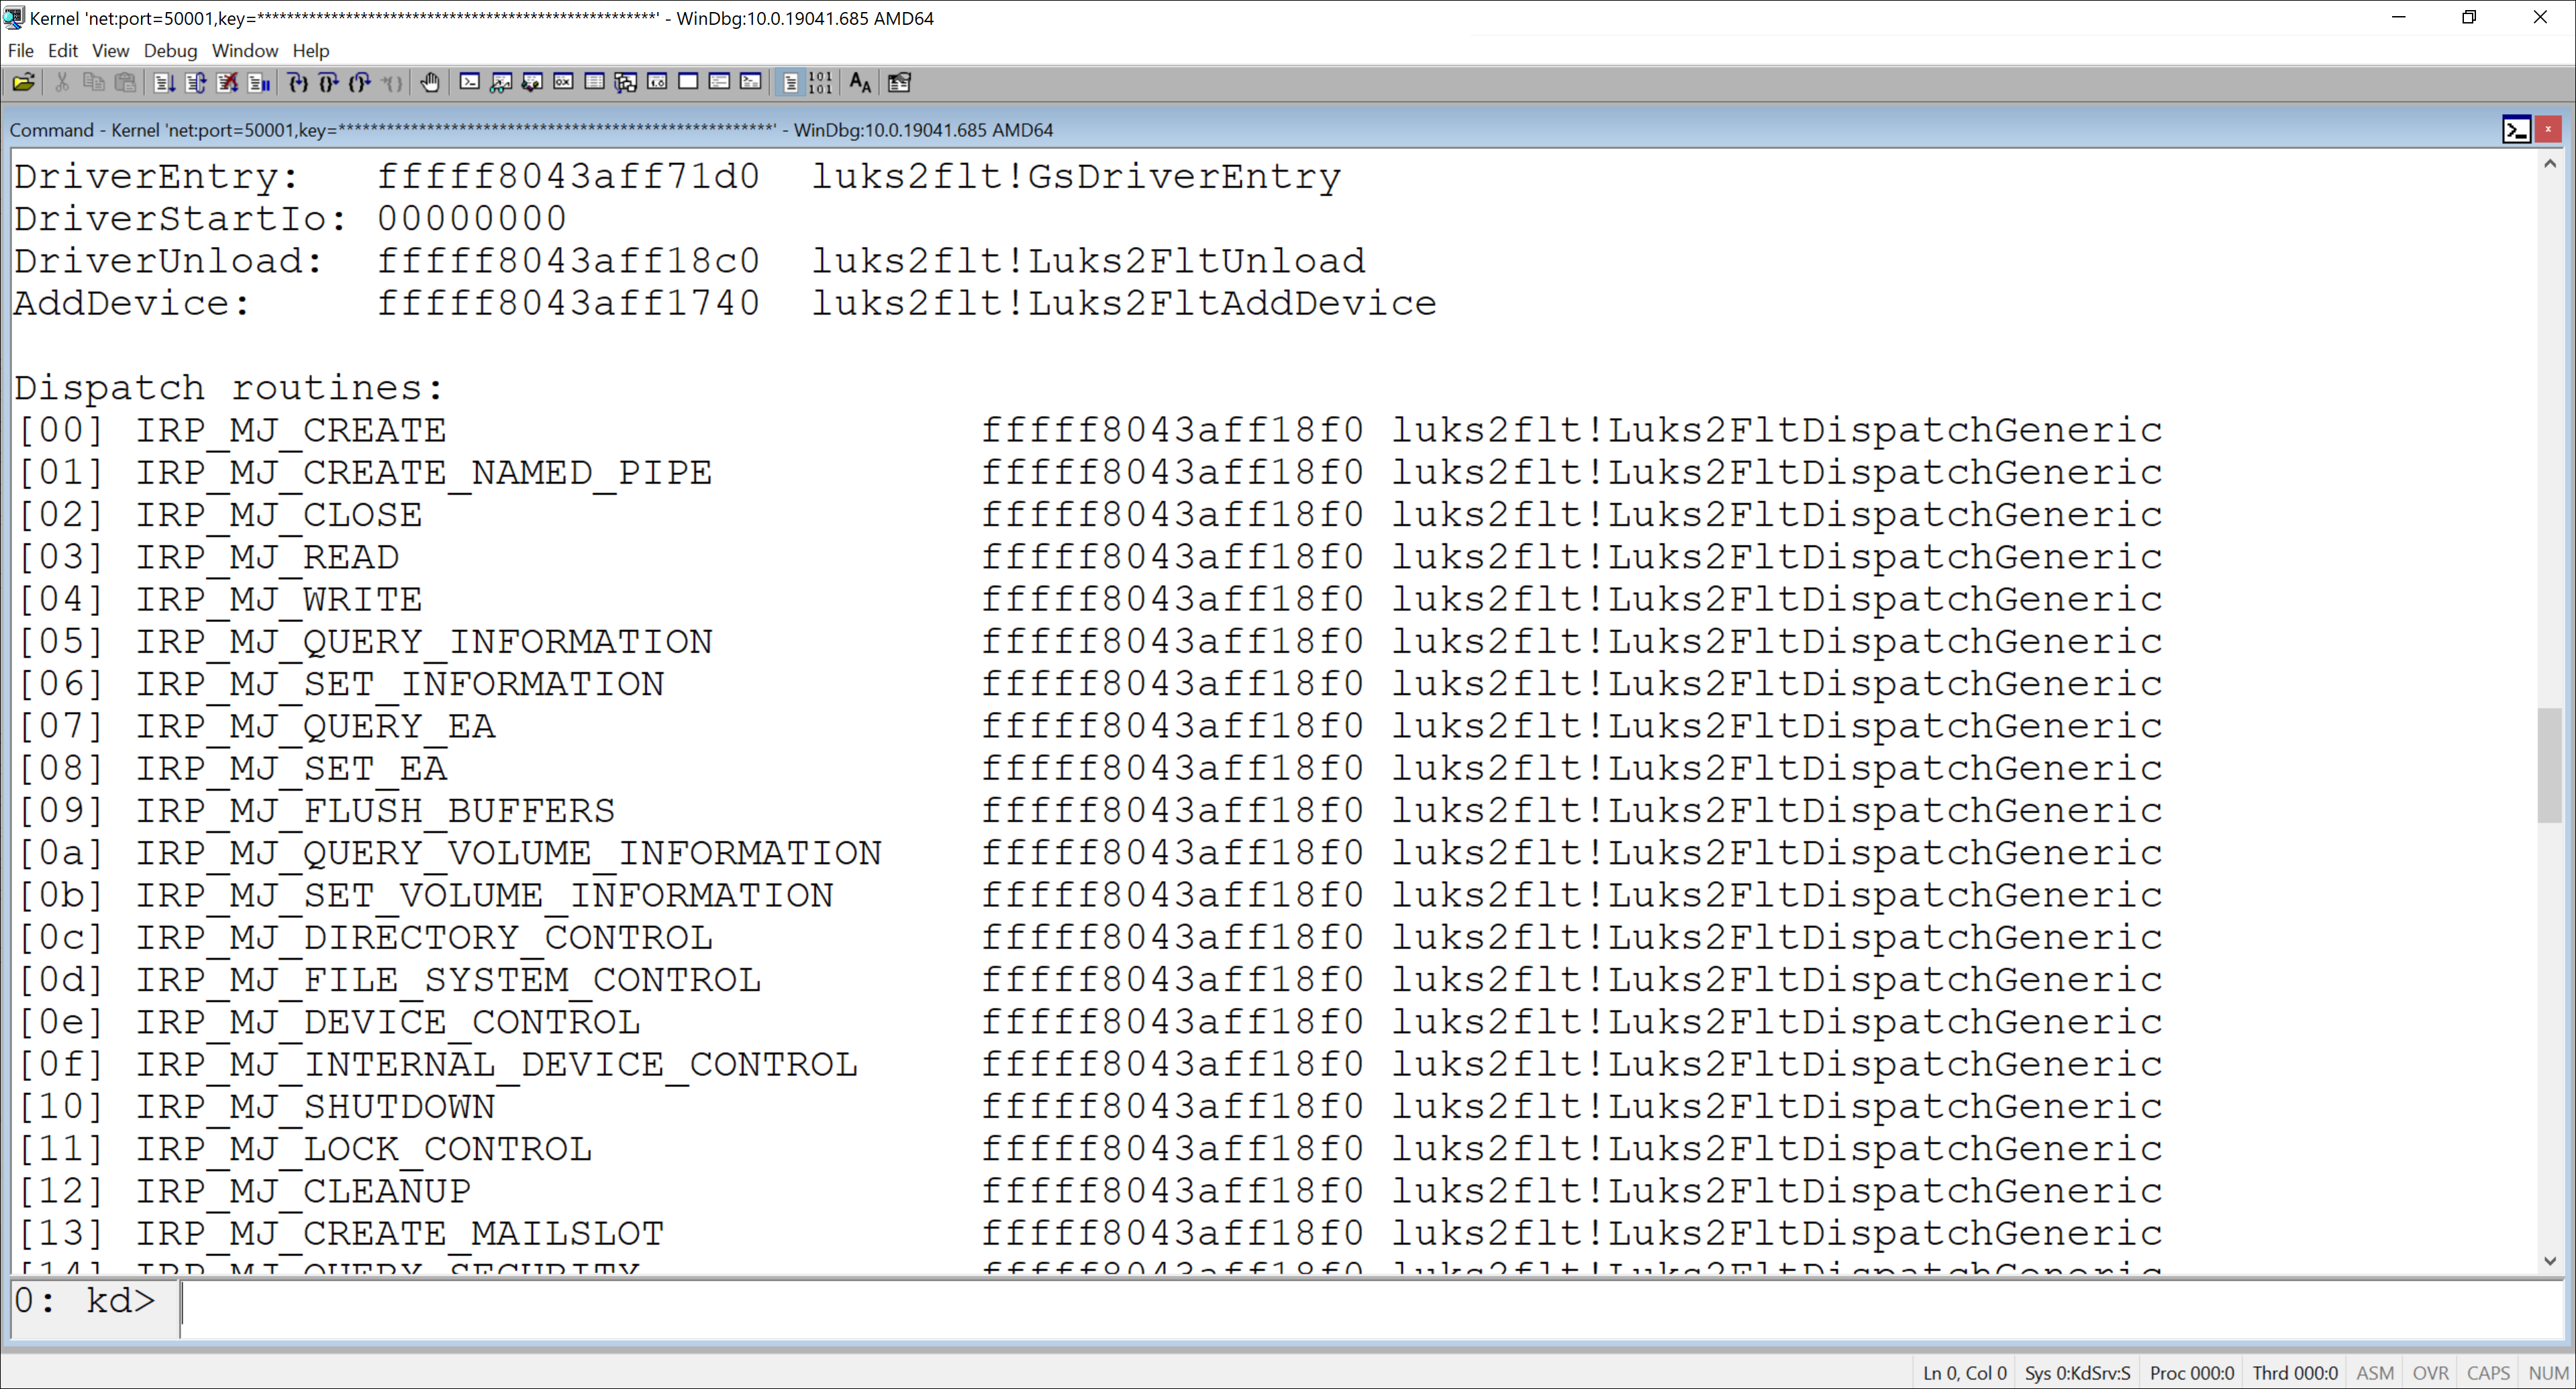
\includegraphics[scale=0.35]{../img/ourapproach.final.windbgdispatch.png}
	\caption[
		\texttt{luks2flt}'s registered routines
	]{
		\texttt{luks2flt}'s registered routines (Screenshot from WinDbg). This is part of the output that WinDbg shows for the \texttt{!drvobj luks2flt 7} command. The routines that were registered during initialization are shown: its unload, \texttt{AddDevice}, and IRP dispatch routines. IRPs of all major functions are handled by a generic dispatch routine, whose logic is described in \autoref{fig:ourapproach.final.irpdispatch}.
	}
	\label{fig:ourapproach.final.windbgdispatch}
\end{figure}

\begin{figure}
	\center
	\small
	\begin{tikzpicture}[
		rect/.append style={
			inner sep=0pt,
			text depth=0pt,
		},
	]
		\node                                                                       (irp)  at (3.7, 4)  {IRP};
		\node[rect, fill=tPink, text width=9em, minimum height=0.8cm]               (gen)  at (8.1, 4)  {\texttt{DispatchGeneric}};
		\node[rect, fill=tOrng, text width=11em, minimum height=0.8cm, anchor=east] (pass) at (16.2, 4) {\texttt{DispatchPassthrough}};

		\foreach \x\n\c in {0/DispatchRead/tYlow,3.3/DispatchWrite/gray!30,6.6/DispatchPower/tYlow,9.9/DispatchPnp/tYlow,13.2/FailIrp/tPurp} {
			\node[rect, fill=\c, from={\x, 1 to \x+3, 1.8}] {\texttt{\n}};
		}
		\foreach \x\n in {1.5/Cleanup,6/CreateClose,10.5/DevControl} {
			\node[rect, fill=tYlow, from={\x, 0 to \x+4.2, 0.8}] {\texttt{Dispatch\n}};
		}
		\draw[dashed] (-0.2, -0.2) rectangle (16.4, 2);

		\draw[arrow] (irp) -> (gen);
		\draw[arrow] (gen) -> node[midway, anchor=south, yshift=-1pt] {\textit{filtering}} (pass);
		\draw[draw=none] (gen) -> node[midway, anchor=north] {\textit{disabled}} (pass);
		\draw[arrow] (gen) -> node[midway, anchor=west, align=left, xshift=1.5pt] {\textit{filtering}\\\textit{enabled}} (8.1, 2);
	\end{tikzpicture}
	\caption[
		IRP flow through \texttt{luks2flt}'s dispatch routines
	]{
		IRP flow through \texttt{luks2flt}'s dispatch routines. All IRPs first arrive at the generic dispatch routine. If filtering has not been enabled for the device, all IRPs (except for two special cases described shortly) are passed on to the next-lower driver in the device stack. If it has been enabled, IRPs that have a dispatch routine corresponding to their major function are sent to this routine. All other IRPs are rejected.\\
		\texttt{DispatchWrite} is greyed out because while an implementation exists, we disabled write access and fail Write IRPs. See \autoref{chap:ourapproach.final.writeproblem} for the reasons why we made this decision.\\
		If a PnP remove request or the IOCTL send by \texttt{luks2filterstart.exe} arrives, it is always handled by \texttt{DispatchPnp} or \texttt{DispatchDevControl}, respectively. These routines for filtered devices already implement handling those requests, and their implementations work just as well for non-filtered devices.
	}
	\label{fig:ourapproach.final.irpdispatch}
\end{figure}

The handling of IRPs with allowed major functions for filtered devices will be described in the following \todo{two} sections.

\subsection{Handling Read and Write Requests}
\label{chap:ourapproach.final.de_encrypting}
The basic idea of handling Read and Write IRPs for filtered volumes is, as we will see, almost the same. We will first describe the commonalities, then the specifics for Write requests, and then those for Read requests (which only require a little modification of the Write process).

Both Read and Write IRPs need adjusting to the read/write offset: all drivers above \texttt{luks2flt} and all user mode applications use offsets relative to the segment's first sector. The drivers below however use offsets relative to the volume's first sector. Therefore, \texttt{luks2flt} needs to translate between those two kinds of offsets. This is as simple as shifting the offset by the position of the encrypted segment on disk.

An example: a program in user mode wants to read the first sector of an unlocked LUKS2 volume. This request reaches \texttt{luks2flt} as a Read IRP with an offset of zero bytes. On disk however there are (in this example) 16 mebibytes of LUKS2 metadata before the first sector of encrypted data. The read offset therefore needs to be set to 16,777,216 bytes, so that the lower-level drivers read the correct, wanted data.

For Write requests, only one more task needs to be done: encrypting the received plaintext data before it is written to disk. Recall from \autoref{chap:background.luks2.using} that LUKS2 supports many encryption algorithms, but \texttt{luks2flt} only supports \texttt{aes-xts-plain64}. The encryption is therefore always done using our own implementation of AES-XTS (\todo{todo}).

Read requests require one more step, because when the IRP first arrives at our driver, no data has actually been read yet. That is the duty of the drivers below \texttt{luks2flt} in the volume's device stack. We therefore need to wait until these have completed all their work for this IRP. Completion routines, which were introduced in \autoref{chap:background.kerneldriver.concepts}, were explicitly designed for this purpose. After shifting the read offset as explained above, the Read dispatch routine registers a completion routine. It will be called when the lower-level drivers have successfully completed the IRP.\footnote{\label{fn:ourapproach.final.failedlowerlevel} Should a lower-level driver fail the IRP, our completion routine will not be called, as there is nothing to decrypt.} The only job of the completion routine is to decrypt the read data. Again, this is accomplished using our AES-XTS implementation.

To minimize the probability of errors, we did not implement all cryptographic algorithms from scratch. Instead, we adapted the AES and AES-XTS implementations of two existing Rust libraries,\footnote{\label{fn:ourapproach.final.rustcrypto} \url{https://github.com/RustCrypto/Block-ciphers} and \url{https://github.com/pheki/Xts-mode}} translating them to C code.

The AES implementation makes use of specific hardware support for AES in CPUs, which was first introduced in 2010 \cite{Intelaes}. This makes it faster than a software-only implementation of AES. Because LUKS2 only uses AES-128 or AES-256, we only implemented these two, and did not implement AES-192.

The AES-XTS implementation builds on AES and provides an interface to encrypt or decrypt one sector of data\footnote{\label{fn:ourapproach.final.blockvssector} Recall from \autoref{chap:background.luks2.using} that AES operates on blocks of 16 bytes. AES-XTS however operates on sectors of arbitrary (but constant for a given device) length; the only requirement is that the sector size is greater than or equal to the block size \cite{Ieee2019}.} at a time, together with a provided tweak.

Using the AES-XTS functions requires previous initialization of an \texttt{Xts} struct, which stores metadata required for en- and decryption. This includes the key, transformed into a representation that can be used by the AES algorithm. Because this struct only needs to be initialized once, this happens when the IOCTL that tells \texttt{luks2flt} to start filtering arrives. \autoref{fig:ourapproach.final.decryptread} shows the usage of the implementation for decrypting one or more sectors read from disk.

\begin{figure}
	\begin{ccode}
VOID
DecryptReadBuffer(
    PUINT8 Buffer,
    PLUKS2_VOLUME_INFO VolInfo,
    PLUKS2_VOLUME_CRYPTO CryptoInfo,
    UINT64 OrigByteOffset,
    UINT64 Length
) {
    UINT64 Sector = OrigByteOffset / VolInfo->SectorSize;
    UINT64 Offset = 0;
    UINT8 Tweak[16];

    while (Offset < Length) {
        ToLeBytes(Sector, Tweak);
        CryptoInfo->Decrypt(
            &CryptoInfo->Xts, Buffer + Offset,
            VolInfo->SectorSize, Tweak
        );
        Offset += VolInfo->SectorSize;
        Sector += 1;
    }
}
	\end{ccode}
	\caption[
		Using our AES-XTS implementation to decrypt read sectors
	]{
		Using our AES-XTS implementation to decrypt read sectors. \texttt{VolInfo} stores the information received in \texttt{luks2filterstart.exe}'s IOCTL, as described in \autoref{chap:ourapproach.final.init}. \texttt{CryptoInfo} stores the aforementioned \texttt{Xts} structure, which holds all data required for cryptographic operations with a given key, plus two function pointers to a \texttt{Decrypt} and \texttt{Encrypt} routine. The functions these point to depend on which key size (128 or 256 bits) is used. \texttt{OrigByteOffset} is the offset that the Read IRP originally contained (as opposed to the offset stored after \texttt{luks2flt}'s modifications). The \texttt{ToLeBytes} function converts the sector number to its 64-bit little-endian representation (this was introduced as the ``plain64'' IV generator in \autoref{chap:background.luks2.using}).
	}
	\label{fig:ourapproach.final.decryptread}
\end{figure}

\subsection{Handling Other Request Types}
\label{chap:ourapproach.final.otherrequests}
Although Read and Write IRPs are the most important and interesting, some other IRP types also need to be supported for the driver to work. In this section, we will describe our approach to handling these other requests when filtering is active. All IRPs with major functions that are not explicitly mentioned in the following are rejected by \texttt{luks2flt}.

\paragraph{Device Control Requests} The dispatch routine for device control requests handles and responds to all IOCTLs that might be sent to a volume. There are a lot of different IOCTLs\footnote{\label{fn:ourapproach.final.ioctls} See \url{http://ioctls.net} for an unofficial list. The IOCTLs starting with \texttt{IOCTL\_DISK}, \texttt{IOCTL\_STORAGE}, \texttt{IOCTL\_VOLUME}, and \texttt{IOCTL\_MOUNTDEV} are relevant for volume devices.}, which makes this a tedious task.\footnote{\label{fn:ourapproach.final.veracryptioctls} The Device Control dispatch routine of the VeraCrypt driver stretches over 1,000 lines of code and handles 38 different IOCTLs (l. 833 to 1889 in \texttt{src/Driver/Ntdriver.c}).} Aside from handling the aforementioned IOCTL sent by \texttt{luks2filterstart.exe}, \texttt{IOCTL\_DISK\_SET\_LUKS2\_INFO}, we only implemented support for the IOCTLs that seemed to be necessary for the volume to function correctly.

If \texttt{luks2flt} receives \texttt{IOCTL\_DISK\_GET\_LENGTH\_INFO}, \texttt{IOCTL\_DISK\_GET\_PARTITION\_INFO}, \texttt{IOCTL\_DISK\_GET\_PARTITION\_INFO\_EX}, or \texttt{IOCTL\_VOLUME\_GET\_VOLUME\_DISK\_EXTENTS}, it registers a completion routine. The responses to all of these include information about the starting offset and/or length of the volume. The offset and length of the decrypted data on disk are different from the values for the underlying volume because of the LUKS2 metadata. The completion routine therefore modifies these values in the responses sent by the lower-level drivers.

We also investigated part of the other IOCTLs that our driver received, and identified some that we believe do not require intervention or modification.\footnote{\label{fn:ourapproach.final.unproblematicioctls} See the \texttt{Luks2FltDispatchDeviceControl} routine in the source code.} These are therefore allowed to pass through. All other IOCTLs are blocked to prevent false information being sent by a lower-level driver.

\paragraph{PnP Requests} The PnP manager notifies drivers about PnP events through IRPs with the \texttt{IRP\_MJ\_PNP} major function. These are sent e.g. during device enumeration or when a device is (about to be) removed from the computer. The exact request type is specified in the IRP's minor function code \cite{Kerneldriver}.

Some of the existing minor function codes must be supported by all (non-legacy) WDM drivers, others are optional \cite{Kerneldriver}. We chose to ignore all optional requests (i.e. just pass them to the next driver), and handle the required ones as follows:
\begin{itemize}
	\item Devices can be started, stopped and restarted by the PnP manager. This has to do with hardware initialization and resource allocation, e.g. allocating I/O ports. Because \texttt{luks2flt} does not allocate any hardware resources, it more or less ignores the minor functions of this category.\footnote{\label{fn:ourapproach.final.pnpstartstop} Which are \texttt{START\_DEVICE}, \texttt{QUERY\_STOP\_DEVICE}, \texttt{CANCEL\_STOP\_DEVICE}, and \texttt{STOP\_DEVICE}. Also note that between Stop and Start requests, drivers theoretically need to queue all incoming IRPs that must not be dropped. Because our driver has no queuing functionality, we rely on the lower-level drivers to do that.}
	\item Devices can also be removed, e.g. when the user ejects hardware or removes a device without informing the OS about it before.\footnote{\label{fn:ourapproach.final.removeforupdate} Devices are also removed for driver updates and re-added after the new driver version has been loaded.} Drivers can fail remove requests, but \texttt{luks2flt} has no reason to do so. It more or less ignores the requests that warn about imminent removal\footnote{\label{fn:ourapproach.final.removalwarningpnp} \texttt{QUERY\_REMOVE\_DEVICE}, \texttt{CANCEL\_REMOVE\_DEVICE}, and \texttt{SURPRISE\_REMOVAL}. The last one is not really a warning but occurs when hardware is suddenly removed, but it is ignored as well.} and only in reaction to the \texttt{REMOVE\_DEVICE} request it detaches from the device stack and deletes its device object.
	\item The last required minor function is the \texttt{DEVICE\_USAGE\_NOTIFICATION}, which lets a driver know that a device contains a paging, dump, or hibernation file. This may have implications for Stop or Remove requests. \texttt{luks2flt} does not care about this and lets the lower-level drivers decide how such a usage impacts device operation.
\end{itemize}
%
% Required PnP minor function codes in more detail:
%	* START_DEVICE - informs about assigned hardware resources. irrelevant for our driver as we do not care about hardware resources.
%	* QUERY_STOP_DEVICE - ``The PnP manager sends this IRP to query whether a device can be stopped to rebalance resources'' \cite{Kerneldriver}. between STOP_DEVICE and START_DEVICE requests, drivers must queue incoming IRPs if they should not be dropped. we don't do that, but we rely on the lower-level drivers to do it.
%	* CANCEL_STOP_DEVICE - we don't differentiate between different states, therefore we don't do anything in response to this request
%	* STOP_DEVICE - ``a stop IRP is used solely to free a device's hardware resources so they can be reconfigured'' \cite{Kerneldriver} we don't allocalte hardware resources, therefore we don't need to free any.
%	* QUERY_REMOVE_DEVICE - ``inform[s] drivers that a device is about to be removed from the computer and [..] [queries] whether the device can be removed without disrupting the computer. The PnP manager also sends this IRP if a user requests to update driver(s) for the device.'' \cite{Kerneldriver}
%	* CANCEL_REMOVE_DEVICE - informs drivers ``that the device will not be removed'' \cite{Kerneldriver}. drivers must put the device back into the state that it was in before the QUERY_REMOVE_DEVICE request arrived
%	* SURPRISE_REMOVAL - this mostly just means releasing hardware resources and blocking new I/O. detaching from the device stack is only done in response to REMOVE_DEVICE requests.
%	* REMOVE_DEVICE - free hardware resources, pass the IRP down the stack, and afterwards detach from the device stack and free device-specific allocations
%	* DEVICE_USAGE_NOTIFICATION - ``The system sends this IRP when it is creating or deleting a paging file, dump file, or hibernation file'' \cite{Kerneldriver}. We don't care about tehc reation or deletion of paging, crash dump, or hibernation file on a volume. Let the other drivers in the device stack handle this.

\paragraph{Create, Close and Cleanup Requests} A Create request is sent when a handle to a file representing a device (e.g. \texttt{\textbackslash Device\textbackslash HarddiskVolume1}) is requested e.g. by a user mode program. Conversely, the Close and Cleanup requests are sent when the last handle to a device is closed, so that drivers may cancel outstaning requests and deallocate resources. The difference between these two is that Cleanup requests are sent regardless of whether there are any outstanding I/O requests. Close requests are only sent after all outstanding I/O requests have either been cancelled or completed \cite{Kerneldriver}. \texttt{luks2flt} does not impose any restrictions on opening handles and does not allocate any resources for handles. It just passes these requests on to the next driver, which is therefore also responsible for cancelling any outstanding operations. Decompilation of the BitLocker driver shows that, except for some special cases, does the same.

\paragraph{Power, Flush Buffers, Shutdown, and System Control Requests} These are not relevant to our driver and are therefore just passed on to the next driver \cite{Kerneldriver}:
\begin{itemize}
	\item Power requests are sent by the power manager to control the power status of devices.
	\item A Flush Buffer request instructs a driver to flush its internal buffer or the cache of a device.
	\item File system drivers send Shutdown requests to storage device drivers to notify them that the system is about to shut down. In response to this, the data stored in internal data caches will be written to disk before shutdown.
	\item System Control requests are implemented by drivers that use the \emph{Windows Management Instrumentation (WMI)} to provide instrumentation and measurement data.
\end{itemize}

\subsection{The Problem With Writing to a Volume}
\label{chap:ourapproach.final.writeproblem}
\todo{corrupted volume, describe debugging process and findings, include that one photo of}\\\todo{``the file who lived''}

\todo{speculation: the IOCTLs are the reason. although we fail all IOCTLs we don't support. maybe modifying the volume offset is not a good idea?}

\section{Security and Privacy Considerations}
\label{chap:ourapproach.security}
\todo{reference \autoref{chap:otherapproaches.linux}?}

\todo{security:} to communicate with \texttt{luks2flt} (only possible via IOCTLs), a theoretical attacker would need to already have administrator rights. They are required to open a device handle, which is needed for sending IOCTLs. Therefore, any possibly existing security vulnerabilities are of low impact (if an adversary has admin rights, the system is already more or less completely compromised). Of course, we still were careful not to introduce any vulnerabilities.

\todo{privacy:} explain what the other implementations do and that we (could) do the same, but don't do it as consequently. iirc luks2flt zeros out some memory on device deletion?

\todo{\url{https://crates.io/crates/secrecy} for luks2filterstart}

\todo{\cite{Halderman2008} \cite{Guan2018} \cite{Li2021} \cite{Simon2018} for literature on memory disclosure attacks and controlling (memory) side effects}

\todo{\url{https://tails.boum.org/contribute/design/memory_erasure/}}

\todo{\url{https://docs.microsoft.com/en-us/windows-hardware/drivers/ddi/wdm/nf-wdm-rtlsecurezeromemory}}

This is the generic solution written in C for clearing memory of the OpenSSL project (as of version 1.1.1l) \todo{[citation needed], explain \texttt{volatile}?}: \href{https://www.openssl.org/docs/man1.1.1/man3/OPENSSL_cleanse.html}{the doc for it}
\begin{ccode}
/*
 * Pointer to memset is volatile so that compiler must de-reference
 * the pointer and can't assume that it points to any function in
 * particular (such as memset, which it then might further "optimize")
 */
typedef void *(*memset_t)(void *, int, size_t);

static volatile memset_t memset_func = memset;

void OPENSSL_cleanse(void *ptr, size_t len)
{
    memset_func(ptr, 0, len);
}
\end{ccode}
The most popular CPU architectures, including x86, x64, ARM, and SPARC, have a hand-written assembly version of \texttt{OPENSSL\_cleanse}. This avoids the compiler from optimizing the zeroing away.